% !TEX program = lualatex
% !TEX TS-program = lualatex

% Clemson_LaTeX_Accessibility_Talk.tex: the examples from example.tex as
% slides. It's also a good starting point for your own accessible deck.
% Build: latexmk -lualatex Clemson_LaTeX_Accessibility_Talk.tex
% Any frame with \verb or verbatim in it has to be a frame*. The comments in
% each frame are the speaker notes. \pause is fine to use, only the last
% slide of a frame gets tagged.

%------------------------------------------------------------------------------
% METADATA AND CLASS
%------------------------------------------------------------------------------
\DocumentMetadata{
  lang          = en-US,
  pdfstandard   = {UA-2,A-4f},
  tagging       = on,
  check-tagging-status,
}
\documentclass{ltx-talk}

%------------------------------------------------------------------------------
% PACKAGES
%------------------------------------------------------------------------------
\usepackage{booktabs}
\usepackage[version=4]{mhchem}
\usepackage{siunitx}
\usepackage{braket}
\usepackage{algpseudocode}
\usepackage{tikz}
\usepackage{clemson}           % after your other packages
\graphicspath{{resources/}}
\babelprovide[import]{french}

%------------------------------------------------------------------------------
% LOOK
%------------------------------------------------------------------------------
% Change the colors here if you like. Keep text at a 4.5:1 contrast or better
% (white on this purple is 10.3:1, black on the callout is 14.3:1).
\definecolor{clemsonpurple}{HTML}{522D80}
\definecolor{codepanel}{HTML}{F4F0F8}
\definecolor{callout}{HTML}{FFCD82}
\definecolor{structure}{HTML}{FFFFFF}
\pagecolor{clemsonpurple}
\AtBeginDocument{\color{white}}

% Frame titles are white and centered, with no band behind them. The footer
% stays at \small, since Clemson asks for no text under 9 pt.
\EditInstance{header}{std}{color = white, left-hspace = 10mm plus 1fil}
\EditInstance{frametitle}{header}{font = \LARGE\bfseries}
\EditInstance{footer}{std}{font = \small, color = white,
  element-order = {title, framenumber}, separator = \hfill}
\EditInstance{titlepage-element}{title}{font = \huge\bfseries}
\EditInstance{titlepage-element}{subtitle}{font = \Large, before-skip = .5em}
\EditInstance{titlepage-element}{author}{before-skip = 2.5em}
\EditInstance{titlepage-element}{institute}{font = \normalsize}

% code: a light panel for the LaTeX source, verbatim goes inside it.
% \callout{...}: the one thing to remember from a frame.
\newsavebox{\codebox}
\newenvironment{code}
  {\par\noindent\setlength{\fboxsep}{6pt}\begin{lrbox}{\codebox}%
   \begin{minipage}[t]{\dimexpr\linewidth-2\fboxsep\relax}\color{black}\small}
  {\end{minipage}\end{lrbox}\colorbox{codepanel}{\usebox{\codebox}}\par}
\newcommand{\callout}[1]{\par\bigskip
  {\centering\setlength{\fboxsep}{8pt}\colorbox{callout}{%
   \parbox{.85\linewidth}{\centering\color{black}\bfseries #1}}\par}}

\title{Accessible LaTeX with the Clemson package}
\subtitle{Plain LaTeX with one package creating a PDF/UA-2 file}
\author{Clay Morton}
\institute{Clemson University}
\date{}

\begin{document}

\begin{frame}
  \maketitle
\end{frame}

%------------------------------------------------------------------------------
% SETUP
%------------------------------------------------------------------------------
\begin{frame*}
  \frametitle{The Preamble}
  % An untagged PDF looks normal and still fails, and LaTeX won't warn you.
  % This block goes above \documentclass. The package loads hyperref, which
  % is why it comes after your other packages.
  \begin{columns}
    \begin{column}[t]{.42\textwidth}
      \begin{itemize}
        \item \texttt{lang}: the language of the PDF
        \item \texttt{pdfstandard}: PDF/UA-2 and PDF/A-4f
        \item \texttt{tagging}: on, or the build stops
        \item \texttt{check-tagging-status}: a package report in the log
      \end{itemize}
    \end{column}
    \begin{column}[t]{.55\textwidth}
\begin{code}
\begin{verbatim}
\DocumentMetadata{
  lang        = en-US,
  pdfstandard = {ua-2,a-4f},
  tagging     = on,
  check-tagging-status,
}
\documentclass{article}
\usepackage{booktabs}
\usepackage{clemson}
\graphicspath{{resources/}}
\end{verbatim}
\end{code}
    \end{column}
  \end{columns}
  \callout{Load \texttt{clemson} after your other packages.}
\end{frame*}

\begin{frame}
  \frametitle{What the Package Does}
  % The package only fills the gaps, everything else is LaTeX's own
  % tagging.
  \large
  \begin{itemize}
    \item Stops the build if tagging is off
    \item Gives every formula its MathML
    \item Tags the title as the only H1 and moves every heading down a level
    \item Writes Scope and Headers on every table cell
    \item Underlines every link except contents entries and note marks
    \item Sets text ragged right and notes at 9 pt or larger
  \end{itemize}
  \callout{Everything else is plain LaTeX.}
\end{frame}

%------------------------------------------------------------------------------
% TITLE AND HEADINGS
%------------------------------------------------------------------------------
\begin{frame*}
  \frametitle{Title and Headings}
  % Screen reader users move through a document by its headings, so the
  % title is the only H1 and no level gets skipped. The package sets the
  % levels, you just use \section and \subsection in order.
  \begin{columns}
    \begin{column}[t]{.42\textwidth}
      \begin{itemize}
        \item Title: H1
        \item \verb|\section|: H2
        \item \verb|\subsection|: H3
        \item Frame titles in this deck: H2
        \item \verb|\thanks|: a footnote, kept out of the metadata
      \end{itemize}
    \end{column}
    \begin{column}[t]{.55\textwidth}
\begin{code}
\begin{verbatim}
\title{Accessible LaTeX}
\author{First Author\thanks{Corresponding
  author.} \and Second Author}
\date{\today}
\begin{document}
\maketitle
\section{Introduction}
\subsection{Links}
\end{verbatim}
\end{code}
    \end{column}
  \end{columns}
  \callout{One H1, and never skip a level.}
\end{frame*}

%------------------------------------------------------------------------------
% TEXT
%------------------------------------------------------------------------------
\begin{frame*}
  \frametitle{Emphasis and Notes}
  % \emph and \strong are tagged, \textbf only changes how the letters look,
  % so a screen reader never mentions it. Footnotes are tagged as notes.
  \begin{columns}
    \begin{column}[t]{.42\textwidth}
      \emph{Emphasis} and \strong{important text} are tagged, \verb|\textbf|
      is not.\footnote{A footnote, tagged as a note.} Long asides go in an
      endnote.
    \end{column}
    \begin{column}[t]{.55\textwidth}
\begin{code}
\begin{verbatim}
\emph{Emphasis} and
\strong{important text} are tagged.
A footnote.\footnote{A note at
  the foot of the page.}
An aside.\endnote{Printed near
  the end.}
...
\printendnotes
\end{verbatim}
\end{code}
    \end{column}
  \end{columns}
  \callout{Use \texttt{\textbackslash emph} and \texttt{\textbackslash strong}
    when the meaning matters.}
\end{frame*}

\begin{frame*}
  \frametitle{Links}
  % The link text should name where it goes. The package underlines every
  % link except contents entries and note marks, so color is never the only
  % signal.
  \begin{columns}
    \begin{column}[t]{.38\textwidth}
      \href{https://www.clemson.edu/accessibility/}{Clemson Digital
      Accessibility}

      \medskip
      \url{https://www.clemson.edu/}

      \medskip
      \email{first.last@clemson.edu}
    \end{column}
    \begin{column}[t]{.59\textwidth}
\begin{code}
\begin{verbatim}
\href{https://www.clemson.edu/accessibility/}
  {Clemson Digital Accessibility}
\url{https://www.clemson.edu/}
\email{first.last@clemson.edu}
\end{verbatim}
\end{code}
    \end{column}
  \end{columns}
  \callout{Name the destination, never ``click here.''}
\end{frame*}

\begin{frame*}
  \frametitle{Cross-References}
  % \autoref turns the whole phrase into one link, so a screen reader says
  % "Theorem 1" and not just "1". It also stays right when things move.
  \begin{columns}
    \begin{column}[t]{.42\textwidth}
      See \autoref{thm:one} on page~\pageref{thm:one}, \autoref{alg:max} and
      Equation~\eqref{eq:gauss}.
    \end{column}
    \begin{column}[t]{.55\textwidth}
\begin{code}
\begin{verbatim}
See \autoref{thm:one} on
page~\pageref{thm:one},
\autoref{alg:max} and
Equation~\eqref{eq:gauss}.
\end{verbatim}
\end{code}
    \end{column}
  \end{columns}
  \callout{\texttt{\textbackslash autoref} makes the whole phrase the link.}
\end{frame*}

\begin{frame*}
  \frametitle{Lists}
  % Every list item gets a label and a body. enumitem does not work with
  % tagging, so use LaTeX's own label key instead.
  \begin{columns}
    \begin{column}[t]{.42\textwidth}
      \begin{enumerate}[label=(\alph*)]
        \item Lettered items come from a kernel key.
        \item The letters are real labels.
      \end{enumerate}
      \begin{description}
        \item[Alt text] What a picture shows and why it is there.
      \end{description}
    \end{column}
    \begin{column}[t]{.55\textwidth}
\begin{code}
\begin{verbatim}
\begin{enumerate}[label=(\alph*)]
  \item Lettered items come from
    a kernel key.
  \item The letters are real labels.
\end{enumerate}
\begin{description}
  \item[Alt text] What a picture
    shows and why it is there.
\end{description}
\end{verbatim}
\end{code}
    \end{column}
  \end{columns}
  \callout{Use \texttt{label=} for custom labels, not enumitem.}
\end{frame*}

\begin{frame*}
  \frametitle{Quotations and Code}
  % quote is tagged as a block quotation and verbatim is tagged as code,
  % one code line per line. LaTeX does all of this by itself.
  \begin{columns}
    \begin{column}[t]{.42\textwidth}
      \begin{quote}
        Tagging writes down what each part of a document is.
      \end{quote}
      Reserved characters: 100\%, R\&D. A command in a sentence:
      \verb|\emph|.
    \end{column}
    \begin{column}[t]{.55\textwidth}
\begin{code}
\begin{verbatim}
\begin{quote}
  Tagging writes down what each
  part of a document is.
\end{quote}
Reserved characters: 100\%, R\&D.
A command in a sentence: \verb|\emph|.
\end{verbatim}
\end{code}
    \end{column}
  \end{columns}
  \callout{LaTeX tags all of this by itself.}
\end{frame*}

%------------------------------------------------------------------------------
% MATHEMATICS
%------------------------------------------------------------------------------
\begin{frame*}
  \frametitle{Formulas}
  % Every formula goes into the PDF as MathML, so a screen reader can read
  % its structure instead of a string of symbols. Nothing extra to write.
  \begin{columns}
    \begin{column}[t]{.42\textwidth}
      Inline: $e^{i\pi} + 1 = 0$. Displayed, with a label:
      \begin{equation}\label{eq:gauss}
        \int_{-\infty}^{\infty} e^{-x^2}\,dx = \sqrt{\pi}
      \end{equation}
    \end{column}
    \begin{column}[t]{.55\textwidth}
\begin{code}
\begin{verbatim}
Inline: $e^{i\pi} + 1 = 0$.
\begin{equation}\label{eq:gauss}
  \int_{-\infty}^{\infty}
    e^{-x^2}\,dx = \sqrt{\pi}
\end{equation}
\end{verbatim}
\end{code}
    \end{column}
  \end{columns}
  \callout{Every formula is MathML, so a screen reader reads its structure.}
\end{frame*}

\begin{frame*}
  \frametitle{Aligned Steps and Cases}
  % amsmath comes with the package and every line gets its own MathML. A
  % numbered multline warns on every run, so use multline* for now.
  \begin{columns}
    \begin{column}[t]{.42\textwidth}
      \begin{align}
        (a+b)^2 &= a^2 + 2ab + b^2 \\
                &= a^2 + b^2 + 2ab
      \end{align}
      \begin{equation}
        f(x) = \begin{cases} x^2 & x \ge 0 \\ -x & x < 0 \end{cases}
      \end{equation}
    \end{column}
    \begin{column}[t]{.55\textwidth}
\begin{code}
\begin{verbatim}
\begin{align}
  (a+b)^2 &= a^2 + 2ab + b^2 \\
          &= a^2 + b^2 + 2ab
\end{align}
\begin{equation}
  f(x) = \begin{cases}
    x^2 & x \ge 0 \\ -x & x < 0
  \end{cases}
\end{equation}
\end{verbatim}
\end{code}
    \end{column}
  \end{columns}
  \callout{Plain amsmath. Use \texttt{multline*}, not a numbered
    \texttt{multline}.}
\end{frame*}

\begin{frame*}
  \frametitle{What a Formula Means}
  % MathML records how a formula looks, not what it means. An x with a bar
  % is "x bar" whether it's a mean or a complex conjugate, so \MathMLintent
  % adds the meaning. Keep the double braces or the intent is dropped.
  \begin{columns}
    \begin{column}[t]{.42\textwidth}
      Read as ``mean of x'', not ``x bar'':
      \begin{equation}
        \MathMLintent{mean($x)}{{\overline{\MathMLarg{x}{x}}}}
        = \frac{1}{n} \sum_{i=1}^{n} x_i
      \end{equation}
    \end{column}
    \begin{column}[t]{.55\textwidth}
\begin{code}
\begin{verbatim}
\begin{equation}
  \MathMLintent{mean($x)}
    {{\overline{\MathMLarg{x}{x}}}}
  = \frac{1}{n} \sum_{i=1}^{n} x_i
\end{equation}
\end{verbatim}
\end{code}
    \end{column}
  \end{columns}
  \callout{\texttt{\textbackslash MathMLintent} says what a formula means.
    Keep the double braces.}
\end{frame*}

\begin{frame*}
  \frametitle{Chemistry and Units}
  % mhchem, siunitx and braket each turn into a Formula with MathML, just
  % like regular math. Don't load the physics package with them.
  \begin{columns}
    \begin{column}[t]{.42\textwidth}
      Water is $\ce{H2O}$, sulfate is $\ce{SO4^2-}$.

      \medskip
      Standard gravity is \qty{9.81}{\metre\per\second\squared}.

      \medskip
      A state is $\ket{0}$.
    \end{column}
    \begin{column}[t]{.55\textwidth}
\begin{code}
\begin{verbatim}
\usepackage[version=4]{mhchem}
\usepackage{siunitx}
\usepackage{braket}
...
Water is $\ce{H2O}$,
sulfate is $\ce{SO4^2-}$.
\qty{9.81}{\metre\per\second\squared}
A state is $\ket{0}$.
\end{verbatim}
\end{code}
    \end{column}
  \end{columns}
  \callout{These packages tag by themselves. Leave out physics.}
\end{frame*}

\begin{frame*}
  \frametitle{Theorems and Proofs}
  % The package defines theorem, lemma, proposition, corollary, definition,
  % example, remark and algorithm. A proof ends with the word QED, which a
  % screen reader reads, the open square is not read at all.
  \begin{columns}
    \begin{column}[t]{.42\textwidth}
      \begin{theorem}\label{thm:one}
        Every heading in a tagged PDF has a level.
      \end{theorem}
      \begin{proof}
        The package moves every heading one level down.
      \end{proof}
    \end{column}
    \begin{column}[t]{.55\textwidth}
\begin{code}
\begin{verbatim}
\begin{theorem}\label{thm:one}
  Every heading in a tagged PDF
  has a level.
\end{theorem}
\begin{proof}
  The package moves every heading
  one level down.
\end{proof}
\end{verbatim}
\end{code}
    \end{column}
  \end{columns}
  \callout{No \texttt{\textbackslash newtheorem} needed. Proofs end with
    QED.}
\end{frame*}

\begin{frame*}
  \frametitle{Algorithms}
  % The algorithm package does not work with tagging, so algorithm here is
  % a theorem-like block from the package. algpseudocode numbers the steps.
  \begin{columns}
    \begin{column}[t]{.42\textwidth}
      \begin{algorithm}[Find the largest value]\label{alg:max}
        Input: $a_1,\dots,a_n$. Output: the largest of them.
        \begin{algorithmic}[1]
          \State $m \gets a_1$
          \For{$i \gets 2$ to $n$}
            \If{$a_i > m$} \State $m \gets a_i$ \EndIf
          \EndFor
          \State \Return $m$
        \end{algorithmic}
      \end{algorithm}
    \end{column}
    \begin{column}[t]{.55\textwidth}
\begin{code}
\begin{verbatim}
\begin{algorithm}[Find the largest
  value]\label{alg:max}
  Input: $a_1,\dots,a_n$.
  \begin{algorithmic}[1]
    \State $m \gets a_1$
    \For{$i \gets 2$ to $n$}
      \If{$a_i > m$}
        \State $m \gets a_i$
      \EndIf
    \EndFor
    \State \Return $m$
  \end{algorithmic}
\end{algorithm}
\end{verbatim}
\end{code}
    \end{column}
  \end{columns}
  \callout{\texttt{algorithm} is a block from the package, not a float.}
\end{frame*}

%------------------------------------------------------------------------------
% FIGURES
%------------------------------------------------------------------------------
\begin{frame*}
  \frametitle{Alt Text}
  % Without alt text a screen reader skips the picture or reads the file
  % name. Say what it shows and why it's there. The caption goes first,
  % since LaTeX tags the caption first.
  \begin{columns}
    \begin{column}[t]{.42\textwidth}
      \begin{figure}
        \caption{Cables in the store}\label{fig:cables}
        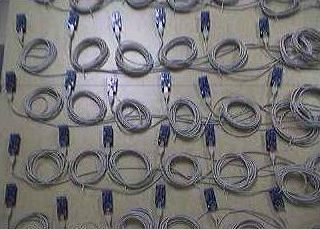
\includegraphics[width=.75\linewidth,alt={Coiled gray cables on a beige pegboard wall.}]{cables}
      \end{figure}
    \end{column}
    \begin{column}[t]{.55\textwidth}
\begin{code}
\begin{verbatim}
\begin{figure}
  \caption{Cables in the store}
  \label{fig:cables}
  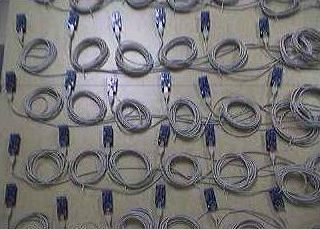
\includegraphics[width=.75\linewidth,
    alt={Coiled gray cables on a
      beige pegboard wall.}]{cables}
\end{figure}
\end{verbatim}
\end{code}
    \end{column}
  \end{columns}
  \callout{Say what the picture shows and why it's there. Caption first.}
\end{frame*}

\begin{frame*}
  \frametitle{Two Panels in One Figure}
  % One caption names the panels and each panel gets its own alt text.
  % subcaption and subfig don't work with tagging, so \hfill places them.
  \begin{columns}
    \begin{column}[t]{.42\textwidth}
      \begin{figure}
        \caption{Two halves of the wall}\label{fig:panels}
        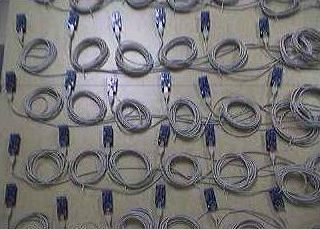
\includegraphics[width=.45\linewidth,trim=0 0 160 0,clip,alt={Panel (a): the left half of the cable wall.}]{cables}
        \hfill
        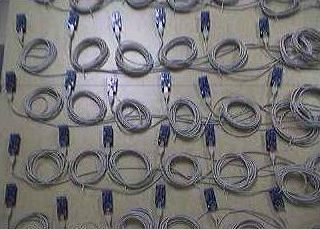
\includegraphics[width=.45\linewidth,trim=160 0 0 0,clip,alt={Panel (b): the right half of the same wall.}]{cables}
      \end{figure}
    \end{column}
    \begin{column}[t]{.55\textwidth}
\begin{code}
\begin{verbatim}
\begin{figure}
  \caption{Two halves of the wall}
  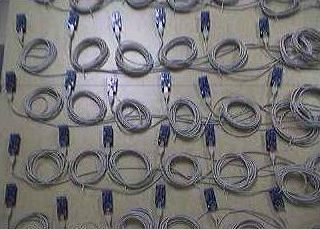
\includegraphics[width=.45\linewidth,
    trim=0 0 160 0, clip,
    alt={Panel (a): the left half
      of the cable wall.}]{cables}
  \hfill
  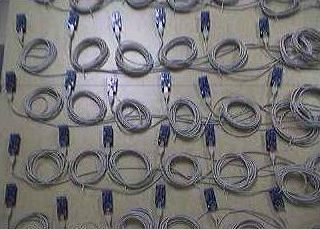
\includegraphics[width=.45\linewidth,
    trim=160 0 0 0, clip,
    alt={Panel (b): the right half
      of the same wall.}]{cables}
\end{figure}
\end{verbatim}
\end{code}
    \end{column}
  \end{columns}
  \callout{One alt text per panel. Skip subcaption and subfig.}
\end{frame*}

\begin{frame*}
  \frametitle{Drawings in the Document}
  % tikzpicture takes the same alt key, so a drawing needs no export step.
  % pgfplots doesn't tag yet, so export a plot as an image instead.
  \begin{columns}
    \begin{column}[t]{.42\textwidth}
      \begin{figure}
        \caption{From source to tagged PDF}\label{fig:tikz}
        \begin{tikzpicture}[alt={Flow diagram: a box labeled LaTeX source, an arrow, and a box labeled tagged PDF.}]
          \draw (0,0) rectangle (2.6,1) node[midway]{LaTeX source};
          \draw[->] (2.7,0.5) -- (3.7,0.5);
          \draw (3.8,0) rectangle (6.2,1) node[midway]{tagged PDF};
        \end{tikzpicture}
      \end{figure}
    \end{column}
    \begin{column}[t]{.55\textwidth}
\begin{code}
\begin{verbatim}
\begin{tikzpicture}[alt={Flow diagram:
  a box labeled LaTeX source, an
  arrow, and a box labeled tagged
  PDF.}]
  \draw (0,0) rectangle (2.6,1)
    node[midway]{LaTeX source};
  \draw[->] (2.7,0.5) -- (3.7,0.5);
  \draw (3.8,0) rectangle (6.2,1)
    node[midway]{tagged PDF};
\end{tikzpicture}
\end{verbatim}
\end{code}
    \end{column}
  \end{columns}
  \callout{\texttt{tikzpicture} takes \texttt{alt} too. Export plots as
    images.}
\end{frame*}

\begin{frame*}
  \frametitle{Pictures of Words and Decoration}
  % Real text is always better. When a logo or a scan has to stay, give it
  % actualtext so a screen reader reads the words. Decoration is an
  % artifact and gets skipped.
  \begin{columns}
    \begin{column}{.42\textwidth}
      \colorbox{white}{\color{black}
\includegraphics[height=0.8cm,actualtext={Clemson University}]{text-image}}

      \bigskip
      \colorbox{white}{\color{black}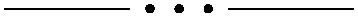
\includegraphics[width=.6\linewidth,artifact]{ornament}}
    \end{column}
    \begin{column}{.55\textwidth}
\begin{code}
\begin{verbatim}

\includegraphics[height=0.8cm,
  actualtext={Clemson University}]
  {text-image}

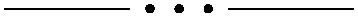
\includegraphics[width=.6\linewidth,
  artifact]{ornament}
\end{verbatim}
\end{code}
    \end{column}
  \end{columns}
  \callout{\texttt{actualtext} gives the words. \texttt{artifact} skips
    decoration.}
\end{frame*}

\begin{frame*}
  \frametitle{Charts}
  % A chart needs more than one sentence. The alt text gives the point and
  % says where the rest is, then the full description and the numbers go in
  % the text where everyone can find them.
  \begin{columns}
    \begin{column}{.42\textwidth}
      \colorbox{white}{\color{black}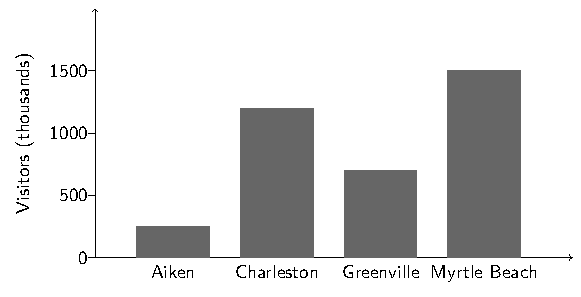
\includegraphics[width=.9\linewidth,alt={Bar chart of visitors to four destinations: Myrtle Beach most, Aiken fewest. Described below.}]{chart}}
    \end{column}
    \begin{column}{.55\textwidth}
\begin{code}
\begin{verbatim}
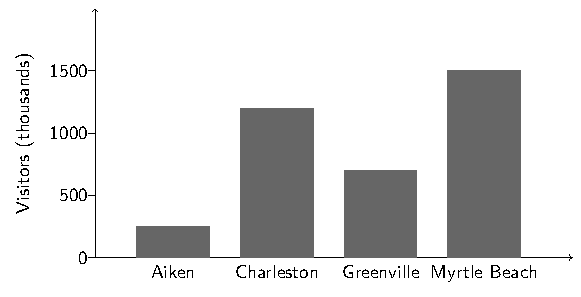
\includegraphics[alt={Bar chart of
  visitors to four destinations:
  Myrtle Beach most, Aiken fewest.
  Described below.}]{chart}
\end{verbatim}
\end{code}

      \medskip
      Aiken had 250 thousand visitors, Charleston 1200, Greenville 700
      and Myrtle Beach 1500.
    \end{column}
  \end{columns}
  \callout{Short alt text, full description in the text.}
\end{frame*}

%------------------------------------------------------------------------------
% OTHER LANGUAGES
%------------------------------------------------------------------------------
\begin{frame*}
  \frametitle{Other Languages}
  % A screen reader only switches voices when the PDF marks the language.
  % Add one \babelprovide line per language after the package. A passage
  % needs a blank line before and after it.
  \begin{columns}
    \begin{column}[t]{.42\textwidth}
      ``Right away'': \foreignlanguage{french}{tout de suite}.

      \begin{otherlanguage}{french}
      Un document accessible porte un arbre de balises que le lecteur
      d'\'ecran suit.
      \end{otherlanguage}
    \end{column}
    \begin{column}[t]{.55\textwidth}
\begin{code}
\begin{verbatim}
\babelprovide[import]{french}
...
\foreignlanguage{french}{tout de suite}

\begin{otherlanguage}{french}
Un document accessible porte un
arbre de balises que le lecteur
d'\'ecran suit.
\end{otherlanguage}
\end{verbatim}
\end{code}
    \end{column}
  \end{columns}
  \callout{Mark the language and the screen reader switches voices.}
\end{frame*}

%------------------------------------------------------------------------------
% TABLES
%------------------------------------------------------------------------------
\begin{frame*}
  \frametitle{A Header Row}
  % Declare the header cells right before \begin{tabular}. Every cell in
  % row 1 becomes a TH with column scope, and the package writes Scope and
  % Headers on every cell so Acrobat and PAC can read them.
  \begin{columns}
    \begin{column}[t]{.42\textwidth}
      \begin{table}
        \caption{Header row}\label{tab:headerrow}
        \tagpdfsetup{table/header-rows={1}}
        \begin{tabular}{lrr}
          \toprule Item & Count & Share \\ \midrule
          Alpha & 12 & 40\% \\
          Beta  & 18 & 60\% \\ \bottomrule
        \end{tabular}
      \end{table}
    \end{column}
    \begin{column}[t]{.55\textwidth}
\begin{code}
\begin{verbatim}
\begin{table}
  \caption{Header row}
  \tagpdfsetup{table/header-rows={1}}
  \begin{tabular}{lrr}
    \toprule Item & Count & Share \\
    \midrule
    Alpha & 12 & 40\% \\
    Beta  & 18 & 60\% \\ \bottomrule
  \end{tabular}
\end{table}
\end{verbatim}
\end{code}
    \end{column}
  \end{columns}
  \callout{Declare the header cells. The package does the rest.}
\end{frame*}

\begin{frame*}
  \frametitle{A Header Column}
  % Every cell in column 1 becomes a TH with row scope. When a table has
  % both, give both keys and the corner cell gets both scopes.
  \begin{columns}
    \begin{column}[t]{.42\textwidth}
      \begin{table}
        \caption{Header column}\label{tab:headercol}
        \tagpdfsetup{table/header-columns={1}}
        \begin{tabular}{lrrr}
          \toprule
          Mean   & 4.1 & 4.4 & 4.0 \\
          Median & 4.0 & 4.5 & 3.9 \\ \bottomrule
        \end{tabular}
      \end{table}
    \end{column}
    \begin{column}[t]{.55\textwidth}
\begin{code}
\begin{verbatim}
\caption{Header column}
\tagpdfsetup{table/header-columns={1}}
\begin{tabular}{lrrr}
  \toprule
  Mean   & 4.1 & 4.4 & 4.0 \\
  Median & 4.0 & 4.5 & 3.9 \\ \bottomrule
\end{tabular}
\end{verbatim}
\end{code}
    \end{column}
  \end{columns}
  \callout{A table with both gets both keys.}
\end{frame*}

\begin{frame*}
  \frametitle{Two Header Rows}
  % Declare both header rows. \multicolumn cells get their column span on
  % their own, and table/multirow=2 lets the corner cell span both rows so
  % there's no empty header under it.
  \begin{columns}
    \begin{column}[t]{.44\textwidth}
      \begin{table}
        \caption{Two-level header}\label{tab:complex}
        \tagpdfsetup{table/header-rows={1,2}, table/header-columns={1}}
        \begin{tabular}{lcccc}
          \toprule
          \tagpdfsetup{table/multirow=2}%
          Method & \multicolumn{2}{c}{Training} & \multicolumn{2}{c}{Test} \\
                 & Prec. & Rec. & Prec. & Rec. \\
          \midrule
          Baseline & 0.74 & 0.68 & 0.71 & 0.64 \\
          Proposed & 0.91 & 0.86 & 0.88 & 0.81 \\ \bottomrule
        \end{tabular}
      \end{table}
    \end{column}
    \begin{column}[t]{.53\textwidth}
\begin{code}
\begin{verbatim}
\tagpdfsetup{table/header-rows={1,2},
  table/header-columns={1}}
\begin{tabular}{lcccc}
  \toprule
  \tagpdfsetup{table/multirow=2}%
  Method & \multicolumn{2}{c}{Training}
         & \multicolumn{2}{c}{Test} \\
         & Prec. & Rec. & Prec. & Rec. \\
  \midrule
  Baseline & 0.74 & 0.68 & 0.71 & 0.64 \\
  Proposed & 0.91 & 0.86 & 0.88 & 0.81 \\
  \bottomrule
\end{tabular}
\end{verbatim}
\end{code}
    \end{column}
  \end{columns}
  \callout{Declare both header rows. \texttt{multirow=2} spans the corner
    cell.}
\end{frame*}

\begin{frame*}
  \frametitle{Side by Side Is Not a Table}
  % A tabular used for layout is read row by row: "First Author Second
  % Author Clemson University Clemson University". A minipage per author is
  % read to its end, so each name stays with its school.
  \begin{columns}
    \begin{column}[t]{.45\textwidth}
      \begin{minipage}[t]{0.48\linewidth}\centering
        First Author\\ Clemson University
      \end{minipage}\hfill
      \begin{minipage}[t]{0.48\linewidth}\centering
        Second Author\\ Clemson University
      \end{minipage}
    \end{column}
    \begin{column}[t]{.52\textwidth}
\begin{code}
\begin{verbatim}
\begin{minipage}[t]{0.48\linewidth}
  \centering
  First Author\\ Clemson University
\end{minipage}\hfill
\begin{minipage}[t]{0.48\linewidth}
  \centering
  Second Author\\ Clemson University
\end{minipage}
\end{verbatim}
\end{code}
    \end{column}
  \end{columns}
  \callout{Tables are for data. Use a minipage for layout.}
\end{frame*}

%------------------------------------------------------------------------------
% CHECKING
%------------------------------------------------------------------------------
\begin{frame*}
  \frametitle{Check the PDF}
  % Acrobat's checker tests PDF/UA-1 and flags "Lbl and LBody" on caption
  % numbers, theorem numbers and note marks. That one is a false positive,
  % don't worry about it.
  Clemson's Digital Accessibility team checks every PDF with Acrobat's
  Accessibility Checker.

  \medskip
  \begin{columns}
    \begin{column}[t]{.42\textwidth}
      Build it:

      \medskip
\begin{code}
\begin{verbatim}
latexmk -lualatex main.tex
\end{verbatim}
\end{code}
    \end{column}
    \begin{column}[t]{.55\textwidth}
      Then check by hand:
      \begin{enumerate}
        \item Alt text says what and why
        \item One H1 and no skipped levels
        \item Header cells declared on every table
        \item Link text names the destination
        \item Color is never the only signal
      \end{enumerate}
    \end{column}
  \end{columns}
  \callout{Then run
    \href{https://www.clemson.edu/accessibility/digital/guides/pdf/check-accessibility/manual-checks.html}{Clemson's
    manual checks} in Acrobat Pro.}
\end{frame*}

%------------------------------------------------------------------------------
% CLOSING
%------------------------------------------------------------------------------
\begin{frame*}
  \frametitle{Getting Started}
  % main.tex is the blank starter and example.tex is the worked example.
  \large
  \begin{enumerate}
    \item Put \verb|\DocumentMetadata| above \verb|\documentclass|, then your
      packages, then \verb|\usepackage{clemson}|
    \item Write plain LaTeX: \verb|\section| in order, \verb|\autoref|,
      \verb|\emph| and \verb|\strong|
    \item Give every picture \texttt{alt} text and every table its header
      cells
    \item Build with latexmk, then run the checks by hand
  \end{enumerate}
  \callout{\url{https://github.com/ClayMorton/Clemson_A11Y_LaTeX}}
\end{frame*}

\begin{frame}
  \frametitle{Resources}
  \large
  \begin{itemize}
    \item \href{https://www.clemson.edu/accessibility/}{Clemson Digital
      Accessibility}
    \item \href{https://latex3.github.io/tagging-project/}{The LaTeX tagging
      project}
    \item \href{https://pdfa.org/resource/best-practice-guide-math-in-pdf/}{PDF
      Association, Best Practice Guide: Math in PDF}
    \item \href{https://pdfa.org/resource/tagged-pdf-best-practice-guide-syntax/}{PDF
      Association, Tagged PDF Best Practice Guide}
  \end{itemize}
\end{frame}

\end{document}
